\chapter{Projekt systemu Team Challenge}

W niniejszym rozdziale przedstawiony został projekt systemu sporządzony na podstawie ogólnej koncepcji opisanej w poprzedniej części. W ramach projektu wydzielono role aktorów na stronie, następnie sporządzono specyfikację wymagań funkcjonalnych. Na podstawie tychże wymagań zostały zamodelowane encje występujące w systemie, co zostało zademonstrowane na diagramie związków encji. W ostatniej części rozdziału przedstawiono diagram stanów dla rzucanego wyzwania.

\section{Role w systemie}

W systemie zostały wyróżnione następujące role. 

\begin{itemize}

\item \textbf{Gość} - Niezalogowana osoba odwiedzająca system.  

\item \textbf{Użytkownik} - Zarejestrowany oraz zalogowany użytkownik systemu.

\item \textbf{Zawodnik} - Użytkownik posiadający profil zawodnika.  

\item \textbf{Kapitan} - Zawodnik, który zarządza własną drużyną. 

\item \textbf{Moderator} - Użytkownik posiadający specjalne uprawnienia. Nadzoruje jakość funkcjonalności dostarczanych przez system. Moderuje wprowadzane obiekty sportowe.    

\item \textbf{Administrator} - Specjalny użytkownik posiadający największe uprawnienia. Ma dostęp do wszystkich danych w systemie. Nadzoruje prawidłowe działanie systemu pod względem technicznym.  

\end{itemize}



\begin{figure}[H]
\centering
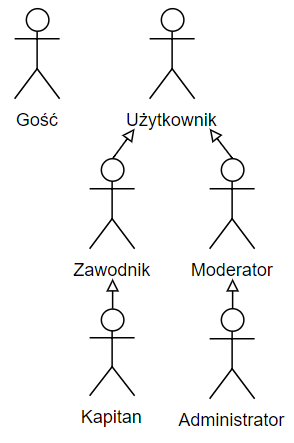
\includegraphics[width=0.25\linewidth]{04-projekt/rys/roles.PNG}
\caption{Diagram zależności między grupami w systemie}
\label{fig:diagram-trad-alg-opt}
\end{figure}


\section{Wymagania funkcjonalne}

Wymagania funkcjonalne zostały zdefiniowane, aby w jasny sposób opisać oczekiwania wobec systemu oraz jego zakres odpowiedzialności. Dokładne definiowanie wymagań pozwala na zidentyfikowanie możliwych błędów koncepcyjnych jeszcze przed rozpoczęciem implementacji \cite{requirements}. Specyfikacja wymagań za pomocą przypadków użycia w sposób czytelny przedstawia możliwe interakcje poszczególnych aktorów z systemem \cite{usecase}.

W poniższych sekcjach przedstawiono diagramy przypadków użycia. W celu poprawienia czytelności, przypadki użycia dla niektórych aktorów zostały przedstawione na oddzielnych diagramach. Dodatkowo dla wybranych spośród najbardziej istotnych przypadków zostały sporządzone szczegółowe opisy.


\subsection{Diagramy przypadków użycia}

\begin{figure}[H]
\centering
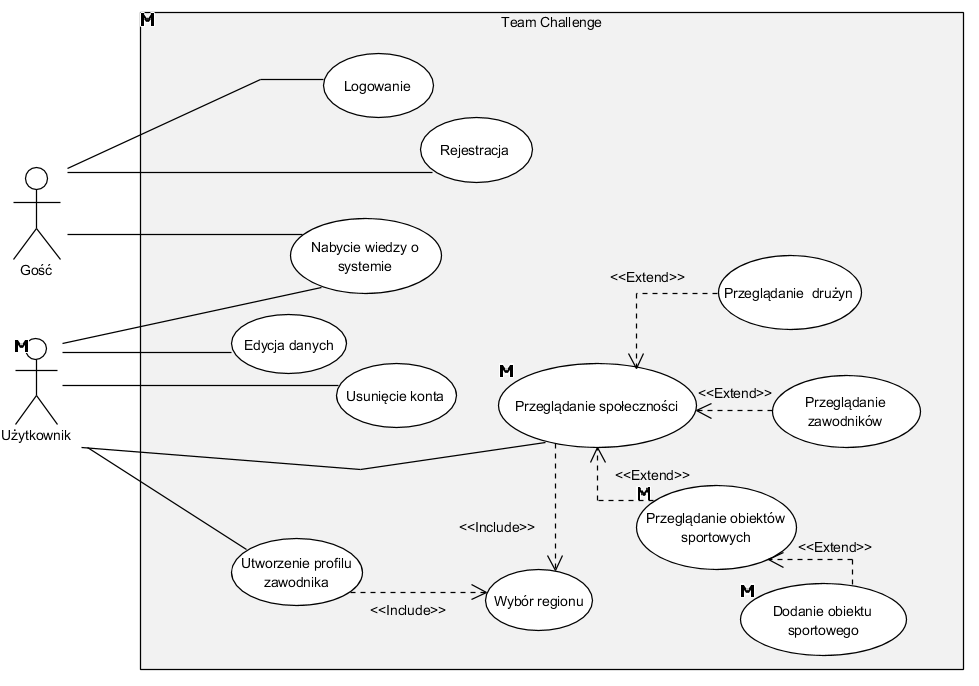
\includegraphics[width=\linewidth]{04-projekt/rys/usecase1.PNG}
\caption{Diagram przypadków użycia - gość oraz użytkownik}
\label{fig:diagram-trad-alg-opt}
\end{figure}

\begin{figure}[H]
\centering
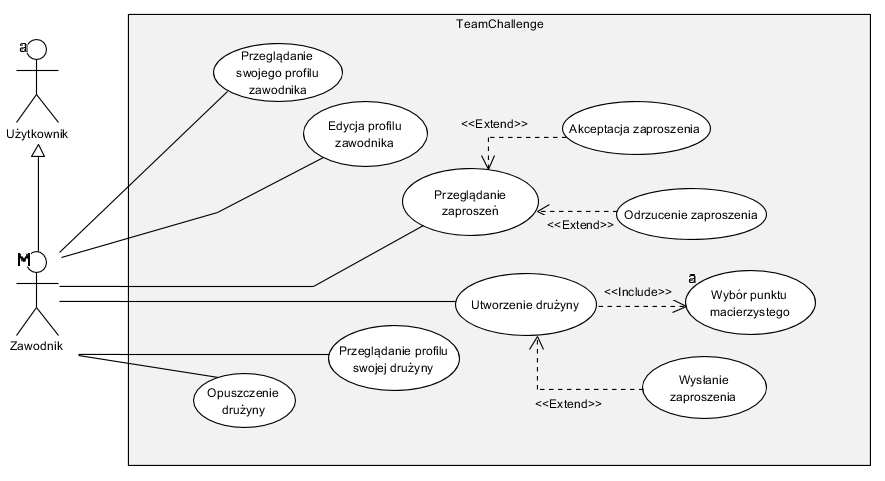
\includegraphics[width=\linewidth]{04-projekt/rys/usecase2.PNG}
\caption{Diagram przypadków użycia - zawodnik}
\label{fig:diagram-trad-alg-opt}
\end{figure}

\begin{figure}[H]
\centering
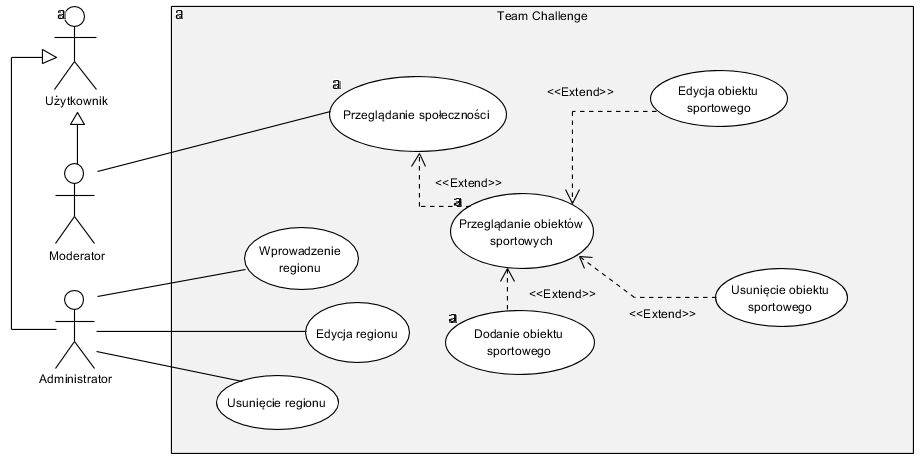
\includegraphics[width=\linewidth]{04-projekt/rys/usecase4.PNG}
\caption{Diagram przypadków użycia - moderator oraz administrator}
\label{fig:diagram-trad-alg-opt}
\end{figure}

\begin{figure}[H]
\centering
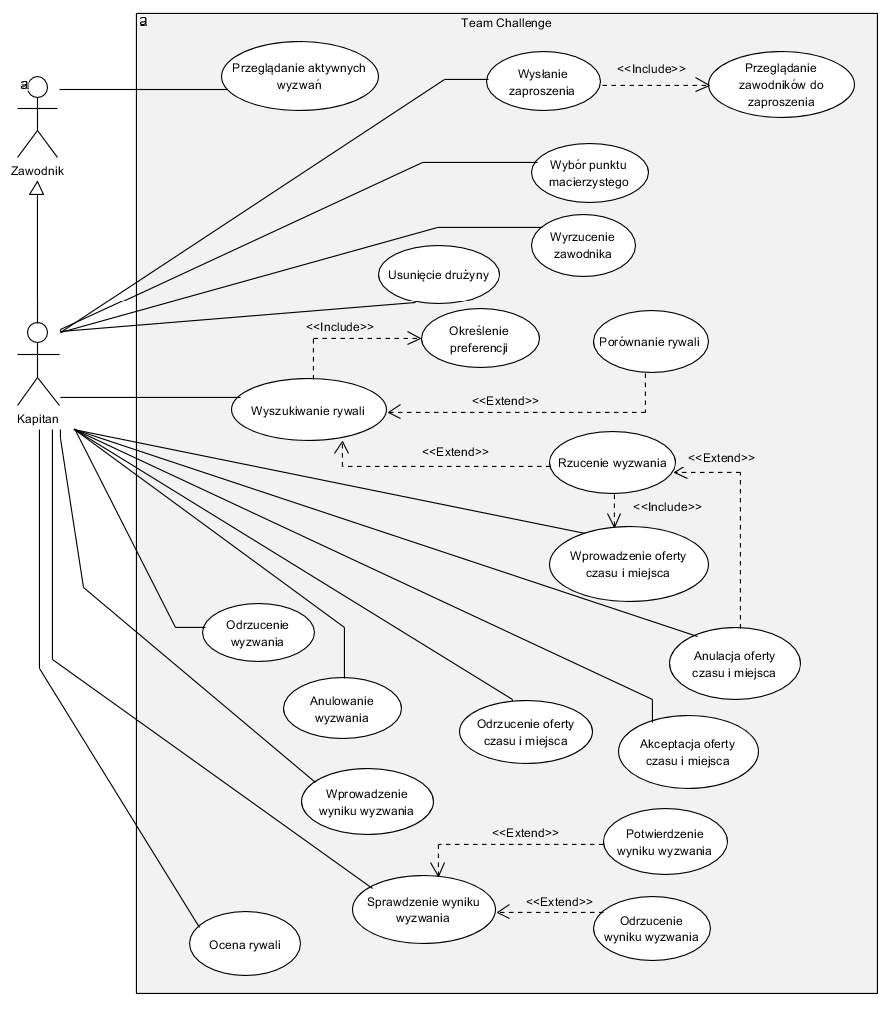
\includegraphics[width=\linewidth]{04-projekt/rys/usecase3.PNG}
\caption{Diagram przypadków użycia - kapitan}
\label{fig:diagram-trad-alg-opt}
\end{figure}


\subsection{PU Rejestracja}

Opis krótki?

\subsubsection{Warunki początkowe}
Gość nie posiadający konta w systemie
\subsubsection{Warunki końcowe}
Konto utworzone w systemie. Możliwe zalogowanie.
\subsubsection{Przebieg}
\begin{enumerate}
  \item System wyświetla formularz rejestracyjny.
  \item Użytkownik wypełnia formularz podając następujące dane: adres e-mail, imię i nazwisko, hasło (dwukrotnie), datę urodzenia.

\end{enumerate}


\begin{table}[H]
\centering\small
\caption{Wymagania funkcjonalne - konta użytkowników}
\label{tab:szablon}
\begin{tabularx}{\linewidth}{|p{.2\linewidth}|X|}\hline
Nr. ident. & Opis \\ \hline\hline

FR-USR-01 & Gość może założyć konto w systemie podając: adres email, hasło, imię, nazwisko oraz datę urodzenia. \\ \hline
FR-USR-02 & Użytkownik może modyfikować wprowadzone przez siebie dane.  \\ \hline
FR-USR-03 & Użytkownik może usunąć swoje konto.  \\ \hline

\end{tabularx}
\end{table}

\subsubsection{Profile zawodników}


\begin{table}[H]
\centering\small
\caption{Wymagania funkcjonalne - profile zawodników}
\label{tab:szablon}
\begin{tabularx}{\linewidth}{|p{.2\linewidth}|X|}\hline
Nr. ident. & Opis \\ \hline\hline

FR-PLR-01 & Użytkownik może utworzyć profil zawodnika. Użytkownik dokonuje wyboru regionu, wprowadza swój wzrost, deklaruje poziom umiejętności oraz częstość gry.   \\ \hline
FR-PLR-02 & Użytkownik może przeglądać swój profil zawodnika.\\ \hline
FR-PLR-03 & Użytkownik może zarządzać swoim profilem zawodnika. \\ \hline

\end{tabularx}
\end{table}

\subsubsection{Dołączanie do drużyn}

\begin{table}[H]
\centering\small
\caption{Wymagania funkcjonalne - dołączanie do drużyn}
\label{tab:szablon}
\begin{tabularx}{\linewidth}{|p{.2\linewidth}|X|}\hline
Nr. ident. & Opis \\ \hline\hline

FR-JOI-01 & Zawodnik nie będący w drużynie może przeglądać otrzymane zaproszenia do drużyn.\\ \hline

FR-JOI-02 & Zawodnik nie będący w drużynie może zaakceptować otrzymane zaproszenie do drużyny.\\ \hline

FR-JOI-03 & Zawodnik nie będący w drużynie może odrzucić otrzymane zaproszenie do drużyny.\\ \hline

FR-JOI-04 & Zawodnik może opuścić drużynę, której jest członkiem, pod warunkiem, że nie jest jej kapitanem.\\ \hline

\end{tabularx}
\end{table}


\subsubsection{Zarządzanie drużynami}

\begin{table}[H]
\centering\small
\caption{Wymagania funkcjonalne - zarządzanie drużynami}
\label{tab:szablon}
\begin{tabularx}{\linewidth}{|p{.2\linewidth}|X|}\hline
Nr. ident. & Opis \\ \hline\hline

FR-TEM-01 & Zawodnik nie będący w drużynie może utworzyć nową drużynę. Zawodnik dokonuje wyboru regionu, wprowadza nazwę oraz wybiera punkt macierzysty.\\ \hline

FR-TEM-02 & Kapitan może dostosować (przenieść) punkt macierzysty swojej drużyny.\\ \hline

FR-TEM-03 & Kapitan może zaprosić do drużyny zawodnika będącego w tym samym regionie co drużyna, pod warunkiem, że nie jest on członkiem żadnej drużyny.\\ \hline

FR-TEM-04 & Kapitan może usuwać zawodników swojej drużyny.\\ \hline

FR-TEM-05 & Kapitan może usunąć swoją drużynę.\\ \hline

FR-TEM-06 & Zawodnik może przeglądać profil swojej drużyny.\\ \hline

\end{tabularx}
\end{table}

\subsubsection{Społeczność}


\begin{table}[H]
\centering\small
\caption{Wymagania funkcjonalne - społeczność}
\label{tab:szablon}
\begin{tabularx}{\linewidth}{|p{.2\linewidth}|X|}\hline
Nr. ident. & Opis \\ \hline\hline

FR-SOC-01 & Użytkownik może przeglądać profile zawodników, drużyn oraz obiekty sportowe w różnych regionach.\\ \hline

FR-SOC-02 & Administrator może dodawać nowe regiony podając ich skrótową nazwę, pełną nazwę oraz wybierając punkt centralny.\\ \hline


\end{tabularx}
\end{table}

\subsubsection{Zarządzanie obiektami sportowymi}

\begin{table}[H]
\centering\small
\caption{Wymagania funkcjonalne - zarządzanie obiektami sportowymi}
\label{tab:szablon}
\begin{tabularx}{\linewidth}{|p{.2\linewidth}|X|}\hline
Nr. ident. & Opis \\ \hline\hline

FR-FAC-01 & Użytkownik może przeglądać mapę z zaznaczonymi obiektami sportowymi w każdym z dostępnych regionów.\\ \hline

FR-FAC-02 & Użytkownik może zgłaszać nowe obiekty sportowe. Użytkownik wskazuje położenie obiektu na mapie oraz wprowadza podstawowe dane takie jak: nazwa, adres, ilość miejsc do gry, nawierzchnia, oświetlenie oraz dodatkowy opis.\\ \hline

FR-FAC-03 & Moderator może usuwać oraz edytować wprowadzone obiekty sportowe.\\ \hline

\end{tabularx}
\end{table}

\subsubsection{Poszukiwanie rywali}

\begin{table}[H]
\centering\small
\caption{Wymagania funkcjonalne - poszukiwanie rywali}
\label{tab:szablon}
\begin{tabularx}{\linewidth}{|p{.2\linewidth}|X|}\hline
Nr. ident. & Opis \\ \hline\hline

FR-SEA-01 & Kapitan aktywnej drużyny może wyszukiwać rywali. \\ \hline

FR-SEA-02 & Kapitan aktywnej drużyny może porównać dwóch lub trzech potencjalnych rywali. \\ \hline

\end{tabularx}
\end{table}


\subsubsection{Organizacja spotkań}

\begin{table}[H]
\centering\small
\caption{Wymagania funkcjonalne - negocjacje}
\label{tab:szablon}
\begin{tabularx}{\linewidth}{|p{.2\linewidth}|X|}\hline
Nr. ident. & Opis \\ \hline\hline

FR-NEG-01 & Kapitan może rzucić wyzwanie innej drużynie  \\ \hline
FR-NEG-02 & Kapitan może anulować wyzwania rzucone przez siebie oraz odrzucać wyzwania rzucone przez inne drużyny  \\ \hline
FR-NEG-03 & Kapitan może odrzucać oferty miejsca i czasu spotkania rzucone przez przeciwników, dodawać oraz wycofywać swoje  \\ \hline
FR-NEG-04 & Kapitan może zaakceptować ofertę miejsca i czasu spotkania rzuconą przez przeciwników. Proces negocjacji dobiega wtedy końca  \\ \hline

\end{tabularx}
\end{table}

\begin{table}[H]
\centering\small
\caption{Wymagania funkcjonalne - wprowadzanie wyniku}
\label{tab:szablon}
\begin{tabularx}{\linewidth}{|p{.2\linewidth}|X|}\hline
Nr. ident. & Opis \\ \hline\hline

FR-RES-01 & Kapitan po spotkaniu może wprowadzić wynik spotkania - wskazać drużynę, która wygrała oraz ilości punktów drużyn  \\ \hline
FR-RES-02 & Kapitan może potwierdzić wynik wprowadzony przez rywali lub go odrzucić w przypadku nieścisłości  \\ \hline
FR-RES-03 & Kapitan może ocenić drużynę przeciwną wypełniając odpowiedni formularz \\ \hline

\end{tabularx}
\end{table}

\section{Identyfikacja encji}

Na podstawie wymagań dotyczących funkcjonowania systemu zidentyfikowane zostały encje.


\begin{table}[H]
\centering\small
\caption{Zestawienie encji wraz z ich opisami}
\label{tab:szablon}
\begin{tabularx}{\linewidth}{|p{.2\linewidth}|X|}\hline
Nazwa encji & Opis \\ \hline\hline

User & Dane użytkownika zarejestrowanego w systemie  \\ \hline
Authority & Poziom uprawnień użytkownika \\ \hline
GrantedAuthority & Encja pomocnicza reprezentująca uprawnienie nadane użytkownikowi \\ \hline
Discipline & Dyscyplina sportu zespołowego \\ \hline
Region & Region, w którym funkcjonuje system  \\ \hline
Position & Punkt na mapie \\ \hline
Player & Dane zawodnika\\ \hline
Team & Dane drużyny\\ \hline
TeamInvitation & Zaproszenie do drużyny wysłane przez kapitana dla zawodnika\\ \hline
Facility & Obiekt sportowy wprowadzony do systemu\\ \hline
Challenge & Wyzwanie pomiędzy dwoma drużynami\\ \hline
ChallengeStatus & Encja pomocnicza reprezentująca status wyzwania\\ \hline
PlaceTimeOffer & Oferta czasu oraz miejsca spotkania utworzona przez jedną z drużyn\\ \hline
PlaceTimeOfferStatus & Encja pomocnicza reprezentująca status oferty czasu oraz miejsca spotkania\\ \hline
Result & Wynik spotkania wprowadzony przez jedną z drużyn\\ \hline
ResultStatus & Encja pomocnicza reprezentująca status wprowadzonego wyniku spotkania\\ \hline
TeamReview & Wypełniony formularz oceny drużyny po zakończonym spotkaniu\\ \hline

\end{tabularx}
\end{table}

\begin{figure}[ht]
\centering
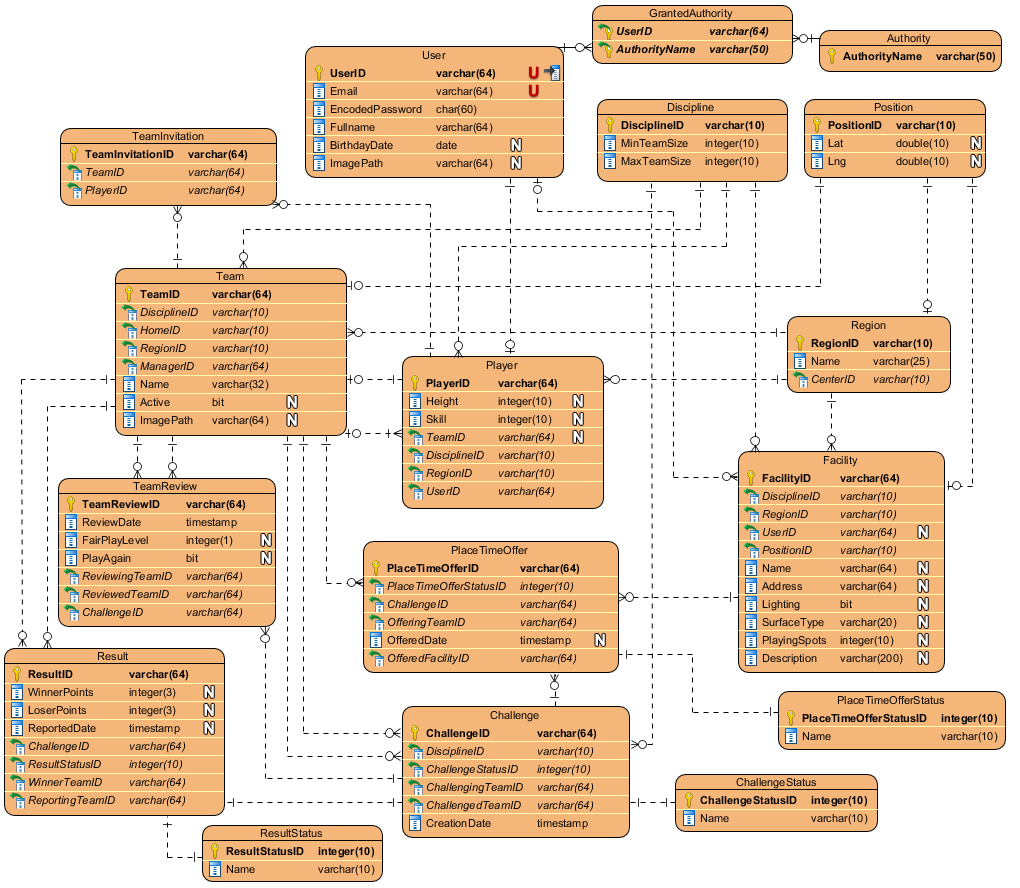
\includegraphics[width=1\linewidth]{04-projekt/rys/erd2.PNG}
\caption{Diagram związków encji}
\label{fig:diagram-erd}
\end{figure}

Encje wraz ze swoimi atrybutami oraz powiązaniami zostały przedstawione w sposób graficzny na rysunku~\ref{fig:diagram-erd} za pomocą diagramu ERD.


Diagram stanów wyzwania??!!


\begin{figure}[H]
\centering
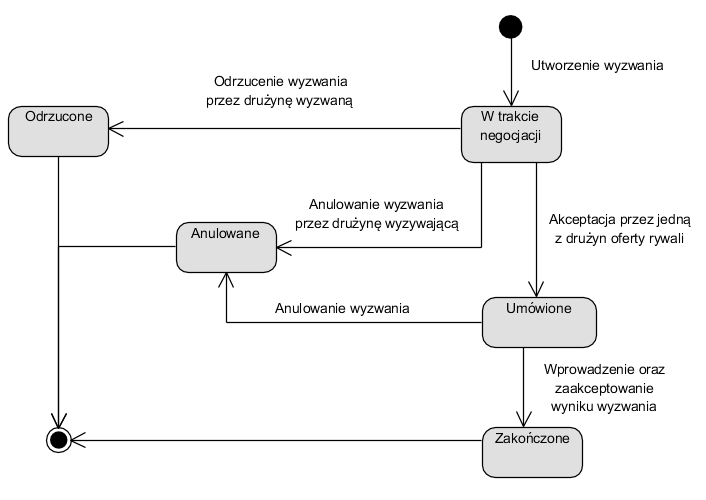
\includegraphics[width=\linewidth]{04-projekt/rys/state1.PNG}
\caption{Diagram zależności między grupami w systemie}
\label{fig:diagram-trad-alg-opt}
\end{figure}



